\documentclass[11pt,a4paper]{article}

\usepackage[applemac]{inputenc}
\usepackage{latexsym}
\usepackage{graphicx}
\usepackage[english]{babel}


\usepackage{amsmath,amssymb}
\usepackage{calc}
\usepackage{multicol}
\usepackage{fancyhdr}
\usepackage{lastpage}
\usepackage[T1]{fontenc}
\usepackage{stmaryrd}
\usepackage[]{algorithm2e}
\usepackage{float}




\begin{document}

\begin{titlepage}
	\title{Optimistic approaches in Contextual Linear Bandit models}
	\author{Mathurin \textsc{Massias} \and Cl�ment \textsc{Nicolle}}
	\date{\today} 
	\maketitle
	\thispagestyle{empty}
	\tableofcontents
\hspace{-6mm}
\end{titlepage}
\newpage
\pagestyle{plain}

\section*{Introduction}

The $K$ multi-arm bandit with partial observation setting is well-studied: at each time $t$, an agent is presented with a fixed set of $K$ arms, from which he chooses one to draw, get a reward $r_t$ (without knowing the rewards he would have obtained pulling another arm), and moves on to $t+1$. The goal of the agent is to maximize its cumulated reward, or to minimize the difference with the cumulated reward he would have had if he had always pulled the best arm.
%
\\[5mm]Here we study a contextual bandit problem, meaning that the set of arms the agent can pull might change over time. For example, we may consider the case of a newspaper website which recommends articles to a user. The arm which is pulled corresponds to the article which is suggested in first position, and the reward depends on if the user clicks on this suggestion. This problem is contextual because over time, the set of available articles can change, and the popularity of an article is likely to decrease as time goes by.
%
\\[5mm]In our problem, we consider that each arm can be described by a vector of $d \in \mathbb{N}^*$ features, which is fixed. In the previous newspaper website example, these features could be the frequencies of some words.
%
\\[3mm]What's more, we study a linear bandit problem: we assume that there exists $\theta \in R^d$ (the same for all arms) such that the reward for pulling arm $i$ at time $t$ is $\theta^{\top} x_i + \epsilon_{t}$, where $\epsilon$ is a centered gaussian noise. Since the noise is uncontrolable, the algorithms focus on estimating $\theta$, to choose the arm with maximal $\theta^{top}x_i$.
\\We consider that $\theta$ is normalized, to simplify the computation of the upper confidence bound. $x_a$s are also normalized, so that adding noise has the same effect on all of them.
%
\\[3mm]To model the change in the set of arms over time, we consider that at each iteration the agent cannot choose amongst all the arms, but only from a fraction of them (denoted $\mathcal{A}_t$, which changes at each iteration, whose cardinal $K$ is a fixed parameter). 
%
\\[5mm]For all our implementations, unless otherwise specified, we have chosen the following parameters :
\\- horizon: $T =10,000$ draws
\\- dimension of the feature space: $d = 100$
\\- total number of arms: N $= 1,000$
\\- number of arms the agent can pull from at each time $t$: K = $100$
\\- probability that the considered concentration inequality holds: $\delta = 0.01$
%TODO how did we chose these ?
%
\\[5mm]What we call regret at iteration $t$ is sometimes called \emph{pseudo-regret} : ${\theta^{\top}(x_{a_t^*} - x_{a_t})}$ where $a_t$ was the arm pulled and $a_t^*$ was the arm maximizing the expected reward (${a_t^* = \mathrm{argmax}_{a \in \mathcal{A}_t} (\theta^{\top} x_a)}$).
\\Since the noise is centered, our regret is just the expectation of the difference between the maximum reward and the reward received. Considering this \emph{pseudo-regret} makes sense: if the noise is independent of the arm selected ($\epsilon_{a,t} = \epsilon_a$), then the noise term cancels out in this difference.
\section{Presentation of LinUCB}

\subsection{Principle}

In all bandit problems, there is a trade-off between exploitation and exploration: to minimize his cumulative regret, the agent must pull the best arm (exploitation), but to do so he must know the best arm (exploration). Pulling all arms uniformly results in a very good knowledge of their distributions, but in poor exploitation, while always pulling the arm which appears best so far ('naive' algorithm) performs badly too, because the best arm can give a poor reward the first time, and never be pulled again.
%
\\[5mm]LinUCB (Linear Upper Confidence Bound) algorithm is derived from the non-contextual algorithm UCB. It is an optimistic algorithm, because it chooses the arms which has the highest upper confidence bound for its mean reward, $\theta^{\top}_a$.
%
\\The principle of this algorithm is, at each iteration, to compute an estimate for $\theta$ and an upper confidence bound for each of the available arms (both based on previous observations), then to pull the arm which has the highest UCB, update the observations made so far, and move to next iteration, where a new estimate of $\theta$ is computed, etc.
%
\\At each iteration $t$, the estimate of $\theta$, $\hat{\theta}_t$, is computed using a linear regression: since for all $s$ in $\llbracket 1, t \rrbracket$, we have $x_s^{\top} \theta = r_s$, left-multiplying each side by $x_s$ and summing for all indices from $1$ to $t$, we have 
%
$$(\sum\limits_{1}^{t}  x_s x_s^{\top} ) \theta =   \sum\limits_{1}^{t} r_s x_s$$
which can be written in matricial form $A_t \theta = b_t$.
\\Using this formula, even if the number of iterations grows, $A_t$ and $b_t$ remain of fixed size. At each iteration we update $A_t$, $b_t$ and the estimate $\hat{\theta}_t = A_t^{-1}b_t$. Since inversing $A_t$ in computationnally costly, we might update it every $k$ iterations only, and thus use the same $\hat{\theta}_t$ for $k$ consecutive iterations.
%
\\[3mm]Initializing $A$ to $I_d$ corresponds to a ridge regression : indeed, if we denote $D_t$ the $t \times d$ design matrix at iteration $t$ : $D_t = \begin{pmatrix} x_1^{\top} \\ ... \\x_t^{\top} \end{pmatrix}$ and $R_t$ the rewards vector $\begin{pmatrix} r_1 \\ ... \\r_t \end{pmatrix}$ , we have: 
%
$$\hat{\theta}_t= (D_t^{\top} D_t + I_d)^{-1} D_t^{\top} R_t$$
which is the formula for a least square ridge regression with regularization parameter equal to 1.
%TODO influence of this parameter ?
%
\\[5mm]The pseudo-code for LinUCB is the following:
\\[3mm]\begin{algorithm}[H]
 \KwData{bandit $\mathcal{A}$, exploration parameter $\alpha$, $K$, horizon $T$}
 $A_1 = I_d$ \;
 $b_1 = 0$ \;
 \For{$t = 1, 2, \ldots, T$}{
  $\hat{\theta}_t = A_t^{-1} b_t$ \;
  Observe $K$ feature vectors: $(x_a)_{a \in \mathcal{A}_t}$ with $\mathcal{A}_t \subset \mathcal{A}$\;
  \For{$a \in \mathcal{A}_t$}{
    $p_{t,a} = \hat{\theta}_t^{\top} x_a + \alpha \sqrt{x_a^{\top}A_t^{-1} x_a}$
   }
   
   Choose arm with higher UCB: $a^*_t = \mathrm{argmax}_{a \in \mathcal{A}_t} p_{t,a} $ \;
   Observe reward $r_t$ \;
   $A_{t+1} = A_t + x_{a^*_t} x_{a^*_t}^{\top}$ \;
   $b_{t+1} = b_t + r_t x_{a^*_t}$ \;
   }
 
  \KwResult{sequences of actions $(a^*_t)$ and payoffs $(r_t)$, $\hat{\theta}_T$}
 \vspace{5mm}
 \caption{LinUCB algorithm}
\end{algorithm}
%
\vspace{5mm}The code can be found in \texttt{linUCB.m}.
%
\subsection{Computation of the UCB}
Since noise is unpredictable, the algorithm only focuses on the expected reward for an arm, $\theta^{\top} x_a$, or equivalently $x_a^{\top} \theta$.
\\Using the previous notations $D_t$ and $R_t$, the difference between the real and estimated rewards at time $t$ for arm $a \in \mathcal{A}_t$ is:
$$\begin{aligned} x_a^{\top} \hat{\theta}_t - x_a^{\top} \theta &= x_a^{\top} A^{-1}_tb_t - x_a^{\top}A_t^{-1} A_t \theta
\\& = x_a^{\top} A^{-1}_t b_t - x_a^{\top}A_t^{-1} (I_d + D^{\top}_tD_t) \theta
\\& = x_a^{\top} A^{-1}_t b_t - x_a^{\top}A_t^{-1} (I_d + D^{\top}_tD_t) \theta
\\& = x_a^{\top} A^{-1}_t D^{\top}_t R_t- x_a^{\top}A_t^{-1} (\theta + D^{\top}_tD_t \theta)
\\& = x_a^{\top} A^{-1}_t D^{\top}_t (R_t - D_t \theta)- x_a^{\top}A_t^{-1} \theta 
\end{aligned}$$
%
Using triangular inequality, Cauchy-Schwarz inequality, $A_t^{\top} = A_t$ and ${\Vert \theta \Vert = 1}$, we get:
$$ \vert x_a^{\top} \hat{\theta}_t - x_a^{\top} \theta \vert \leq \vert x_a^{\top} A^{-1}_t D^{\top}_t (R_t - D_t \theta) \vert + \Vert A^{-1}_t x_a \Vert $$
%
%TODO one is a variance term, other is bias
%
For the second term, we have 
$$\begin{aligned} 
\Vert A^{-1}_t x_a \Vert^2  &= x^{\top}_a A_t^{-1} I_d A_t^{-1} x_a
\\& \leq x^{\top}_a A_t^{-1} (I_d + D_t^{\top}D_t)A_t^{-1} x_a
\\& \leq x^{\top}_a A_t^{-1} x_a
\end{aligned}$$
%
And for the first one, using $\mathbb{E}[R_t - D_t \theta] = 0$ and Azuma's inequality :
$$\begin{aligned} \mathbb{P}( \vert x_a^{\top} A^{-1}_t D^{\top}_t (R_t - D_t \theta) \vert \geq \alpha \sqrt{x^{\top}_a A_t^{-1} x_a})
& \leq 2 \, \mathrm{exp} (- \frac{2 \alpha^2 x^{\top}_a A_t^{-1} x_a}{\Vert D_tA^{-1}_t x_a \Vert ^2})
\\ &\leq 2 e^{-2 \alpha^2}
\\ &= \frac{\delta}{ \mathrm{K}}  % T \,
\end{aligned}$$
Using a union bound for the K possible arms in $\mathcal{A}_t$, we get a uniform bound with probability $1 - \delta$.
\\Combining the bound on the first term and second term, with probability $1 - \delta$, 
$$\vert x_a^{\top} \hat{\theta}_t - x_a^{\top} \theta \vert \leq (1 + \alpha) \sqrt{x^{\top}_a A_t^{-1} x_a}$$
where $\alpha = \sqrt{\frac{\mathrm{log} (2K/\delta)}{2}}$. %TODO there's an extra K here... (K = K)

%
\subsection{Impact of exploration parameter}
The exploration parameter $\alpha$ is related to $\delta$ by $\alpha = 1 + \sqrt{\frac{\mathrm{log \,}(2 / \delta)}{2}}$. As the concentration inequality holds with probability $1 - \delta$, if $\delta \to 0$, then ${\alpha \to \infty}$, meaning that if we want a very high probability to find the observed value in a given set, this set must be very large.
%
The higher $\alpha$, the larger the confidence sets: the algorithm is very 'suspicious' about the value $\hat{\theta}_t^{\top}x_i$, and explores more than with a smaller $\alpha$.
\\On the contrary, $\alpha = 0$ %TODO alpha cannot be lesser than 1 with current formula
corresponds to a naive version, where the arm which is pulled is just the one which has the highest mean of rewards observed so far.
\\[5mm]Here are the regrets obtained for LinUCB, with different $\alpha$s (sampled logarithmically from 0 to 1)

\begin{figure}[H]
\centering
\noindent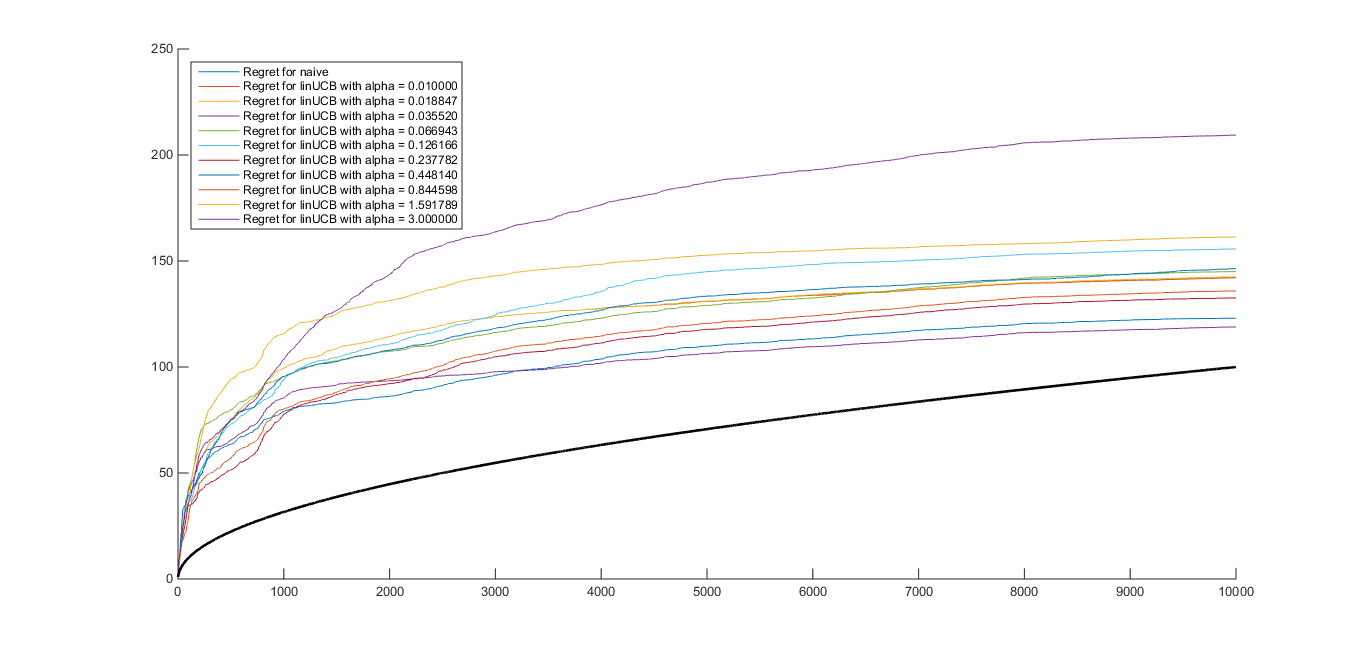
\includegraphics[scale=0.5]{regrets_alphas.png}
\caption{Regret curves for LinUCB with different exploration parameters}
\end{figure}
%TODO mention that this is only one trajectory, but gives an idea of the best alpha. See that low and high alphas perform poorly.
%TODO mention that alpha should change over time.

\section{Comparison with contextual Thompson sampling}


\section{Analysis of OFUL algorithm}
\subsection{Principle}

OFUL (optimism in the face of uncertainty) is also an optimistic algorithm, because it computes a confidence set for $\theta$, and chooses the arm which maximizes the rewards over all $\hat{\theta}_t$ lying in this confidence set.
%
\\The pseudo code for the OFUL algorithm is:
\\\begin{algorithm}[H]
 \KwData{bandit $\mathcal{A}$, exploration parameter $\alpha$, $K$, horizon $T$}
 $A_1 = I_d$ \;
 $b_1 = 0$ \;
 \For{$t = 1, 2, \ldots, T$}{
  $\hat{\theta}_t = A_t^{-1} b_t$ \;
  Randomly select a set $\mathcal{A}_t \subset \mathcal{A}$ of $K$ arms \;
  
  \For{$a \in \mathcal{A}_t$}{
    $p_{t,a} = \hat{\theta}_t^{\top} x_a + f(t,a)$
   }
   
   Choose arm with higher UCB: $a^*_t = \mathrm{argmax}_{a \in \mathcal{A}_t} p_{t,a} $ \; 
   Observe reward $r_t$ \;
   $A_{t+1} = A_t + x_{a^*_t} x_{a^*_t}^{\top}$ \;
   $b_{t+1} = b_t + r_t x_{a^*_t}$ \;
   }
 
  \KwResult{sequences of actions $(a^*_t)$ and payoffs $(r_t)$, $\hat{\theta}_T$}
 \vspace{5mm}
 \caption{OFUL algorithm}
\end{algorithm}
%
\vspace{5mm}
Computing $f(t,a)$ is the key of the algorithm; it is related to the upper bound on the estimated reward for arm $a$ at time $t$. 
\\We have, with probability $1 - \delta$, %TODO quote where this result is from
$$\Vert \hat{\theta}_t - \theta \Vert_{A_t} 
\leq 
\sigma^2 \sqrt{2 \, \mathrm{log} ( \frac{ \vert A_t \vert^{1/2} }{\delta})} + 1$$
Where $\Vert u \Vert_A = \sqrt{u^{\top} M u }$ ($u$ is a $d\times 1$ vector, $M$ is a $d\times d$ matrix).
\\If $A$ is invertible, then for all $u, v$ we have $\vert u^{\top} v \vert \leq \Vert u \Vert_M \Vert v \Vert_{M^{-1}}$, so if we apply this to $M = A^{-1}_t$, $u =x_a$ and $v =  \hat{\theta}_t - \theta$, we get an upper bound on $\vert x_a^{\top} \theta - x_a^{\top} \hat{\theta}_t \vert$ with probability $1-\delta$ : 
$$f(t,a) =  \Vert x_a \Vert_{A^{-1}_t} (\sigma^2 \sqrt{2 \, \mathrm{log} ( \frac{ \vert A_t \vert^{1/2} }{\delta})} + 1)$$
\subsection{Comparison with LinUCB}


%
%
\newpage
\begin{thebibliography}{9}

   \bibitem{}
          Lihong Li,
               Wei Chu,
               John Langford,
               Robert E. Schapire,
          \emph{A Contextual-Bandit Approach to Personalized News Article Recommendation}.
	CoRR, %probably not
          2010.
          \bibitem{}
          Thomas J. Walsh, Istvan Szita, Carlos Diuk, Michael L. Littman,
                    \emph{Exploring compact
reinforcement-learning representations with linear regression}.
	CoRR,
         . %TODO date

\end{thebibliography}

\end{document}